\documentclass[11pt]{article}
\usepackage{amssymb, amsmath, libertine, hyperref, xcolor, booktabs, enumitem, microtype}
\usepackage[T1]{fontenc}
\usepackage[margin=1in]{geometry}
\usepackage{tikz}
\newcommand{\gridxy}[4]{% xmin xmax ymin ymax -- gridlines exactly on the ticks
  \foreach \gX in {#1,...,#2} \draw[gray!25] (\gX,#3) -- (\gX,#4);
  \foreach \gY in {#3,...,#4} \draw[gray!25] (#1,\gY) -- (#2,\gY);}
\definecolor{dark-red}{rgb}{0.4,0.15,0.15}
\definecolor{blue-g}{rgb}{0.15,0.28,0.45}
\hypersetup{colorlinks, linkcolor=dark-red, citecolor=dark-red, urlcolor=dark-red}
\setlist[enumerate,1]{label=\textbf{(\alph*)}, leftmargin=*, itemsep=6pt, topsep=5pt}
\pagestyle{empty}
\newcommand{\prob}[1]{\medskip\noindent\textbf{\large #1}\par\smallskip}
\begin{document}

\begin{center}
{\Large\bfseries Math 111: Calculus \quad Homework 4}\\[4pt]
{Due Friday, November 13 by 10:00\textsc{p.m.} via Gradescope}
\end{center}

\medskip
\noindent\textbf{Covers} Active Calculus \S4.1, \S4.2, \S4.3, and \S5.6. Problems~1 and~3
use \S4.1--\S4.3 and can be done after Wednesday, November~4. Problem~2(a)--(b) uses
\S4.2; Problem~2(c)--(e) and Problem~4 use \S5.6 (Friday, November~6). No problem needs
the Fundamental Theorem of Calculus; if you know it, you may use it to \emph{check} an
answer, but explain each answer the way the problem asks.

\smallskip
\noindent\textbf{Before you start.} Write in sentences and paragraphs, as an
explanation another student in this course could read and follow. Draw diagrams large
and label them. You are encouraged to work with classmates; cite everyone you worked
with, and write your solutions independently --- duplicated solutions are an Honor
Principle violation. Each problem is marked holistically on the 0--5 scale, with up
to two further points for the quality of the writing. If you need an extension, use
the \href{https://docs.google.com/forms/d/e/1FAIpQLSfIfgx44SFtUzefTNr-80yz35MVJaUqQttt96xVTU5mCQCOgg/viewform}{extension
form} \emph{before} the deadline.

\bigskip\hrule\bigskip
\prob{1. A drone's altitude, from its velocity}
A survey drone takes off from a platform and flies straight up and down for ten minutes.
Its vertical velocity $v(t)$, in meters per minute, is graphed below; positive means rising.
The graph is made of straight segments.
\smallskip
\begin{center}
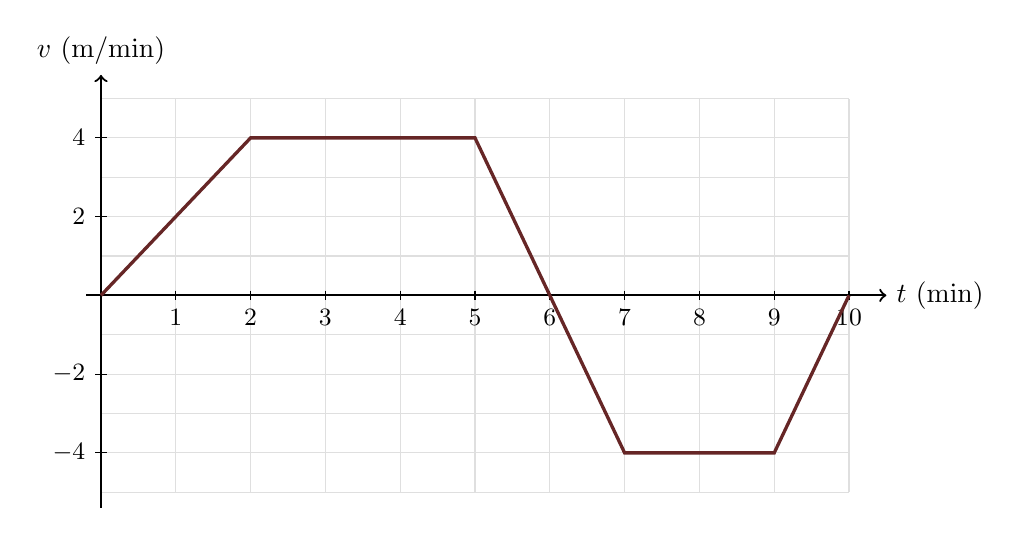
\begin{tikzpicture}[x=0.95cm,y=0.5cm]
  \gridxy{0}{10}{-5}{5}
  \draw[->,thick] (-0.2,0) -- (10.5,0) node[right] {$t$ (min)};
  \draw[->,thick] (0,-5.4) -- (0,5.6) node[above] {$v$ (m/min)};
  \foreach \x in {1,...,10} \draw (\x,0.12) -- (\x,-0.12) node[below,font=\small] {\x};
  \foreach \y in {-4,-2,2,4} \draw (0.08,\y) -- (-0.08,\y) node[left,font=\small] {$\y$};
  \draw[very thick, dark-red] (0,0) -- (2,4) -- (5,4) -- (7,-4) -- (9,-4) -- (10,0);
\end{tikzpicture}
\end{center}
Let $h(t)$ be the drone's height above the platform, in meters, at time $t$, so $h(0)=0$.
\begin{enumerate}
\item On which time intervals is the drone rising, and on which is it falling? How do you know from the graph?

\item How high is the drone at $t=6$? Explain why that is the greatest height it reaches.

\item Where is the drone at $t=10$, relative to the platform?

\item What total distance does the drone travel over the ten minutes? Explain in a sentence why this is not the same as your answer to (c).

\item Find the drone's average velocity over $[0,10]$, with units. Then draw, on a copy of the graph, a horizontal line at that height, and say what the picture shows about the area above and below it.

\item Sketch a graph of $h(t)$ on $[0,10]$. Label the height at $t=2,5,6,7,9,10$. Say where $h$ is concave up, where it is concave down, and where it is a straight line, and say how you read each of those off the graph of $v$.

\end{enumerate}

\newpage
\prob{2. Filling a tank from a table}
Water flows into a tank at a rate $r(t)$, in liters per minute, measured every five minutes:
\smallskip
\begin{center}
\begin{tabular}{@{}lrrrrr@{}}
\toprule
$t$ (min) & 0 & 5 & 10 & 15 & 20\\
$r(t)$ (L/min) & 2 & 3 & 5 & 8 & 12\\
\bottomrule
\end{tabular}
\end{center}
\smallskip
Assume throughout that $r$ is increasing on $[0,20]$. The quantity we want is the amount of
water that flows in over the twenty minutes, $\displaystyle\int_0^{20} r(t)\,dt$.
\begin{enumerate}
\item Compute the left and right sums $L_4$ and $R_4$, with units. Which is an over-estimate and which is an under-estimate? Explain using a picture, not a rule.

\item Explain why, for an increasing $r$ and $n$ equal subintervals, $R_n-L_n=\dfrac{20}{n}\big(r(20)-r(0)\big)$. Then suppose the rate could be measured as often as you like. How many equal subintervals would guarantee that the average $\tfrac12(L_n+R_n)$ is within $1$ liter of the true amount? How often is that, in seconds?

\item Compute the trapezoid estimate $T_4$. The table suggests $r$ is concave up (look at the differences). Assuming it is, is $T_4$ too big or too small? Explain by drawing the graph of $r$ over a single subinterval together with the trapezoid on that subinterval.

\item Use the readings at $t=5$ and $t=15$ to compute the midpoint estimate $M_2$ (two subintervals of width $10$). Assuming $r$ is concave up, is $M_2$ too big or too small? Explain by drawing the graph of $r$ over a single subinterval together with the midpoint rectangle on that subinterval. What interval does your work in (c) and (d) trap the true amount in?

\item Compute $T_2$, and then Simpson's estimate $S=\dfrac{2M_2+T_2}{3}$. Does it land in your interval from (d)? In a sentence or two, explain why combining $M$ and $T$ with these weights should be better than either one alone.

\end{enumerate}

\newpage
\prob{3. Integrals you can read off a picture}
The function $f$ on $[0,6]$ is graphed below. On $[0,2]$ it is a straight line; on $[2,6]$
it is the lower half of a circle of radius $2$ centered at $(4,0)$.
\smallskip
\begin{center}
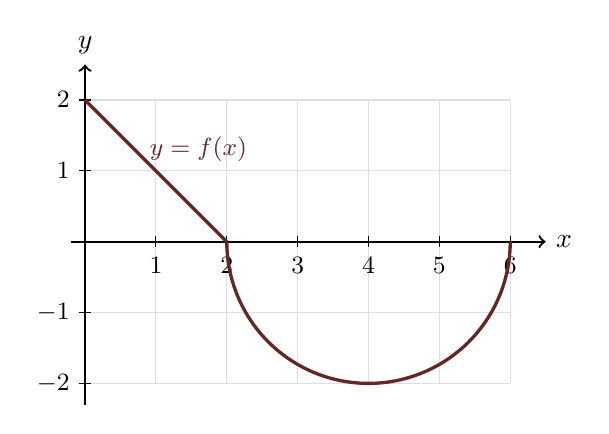
\begin{tikzpicture}[x=0.9cm,y=0.9cm]
  \gridxy{0}{6}{-2}{2}
  \draw[->,thick] (-0.2,0) -- (6.5,0) node[right] {$x$};
  \draw[->,thick] (0,-2.3) -- (0,2.5) node[above] {$y$};
  \foreach \x in {1,...,6} \draw (\x,0.08) -- (\x,-0.08) node[below,font=\small] {\x};
  \foreach \y in {-2,-1,1,2} \draw (0.08,\y) -- (-0.08,\y) node[left,font=\small] {$\y$};
  \draw[very thick, dark-red] (0,2) -- (2,0);
  \draw[very thick, dark-red, domain=180:360, samples=80] plot ({4+2*cos(\x)},{2*sin(\x)});
  \node[dark-red,font=\small] at (1.6,1.3) {$y=f(x)$};
\end{tikzpicture}
\end{center}
Use geometry and the properties of the definite integral; no Riemann sums are needed.
\begin{enumerate}
\item Find $\displaystyle\int_0^2 f(x)\,dx$, $\displaystyle\int_2^6 f(x)\,dx$, and $\displaystyle\int_0^6 f(x)\,dx$. Explain why one of them is negative.

\item Find $\displaystyle\int_0^6 |f(x)|\,dx$ and $\displaystyle\int_6^0 f(x)\,dx$.

\item Find $\displaystyle\int_0^6 \big(3f(x)+1\big)\,dx$. Say which properties of the integral you used.

\item Find the average value of $f$ on $[0,6]$. Is it positive or negative? Explain in a sentence why that matches the picture.

\item Suppose $f(x)$ is the rate, in thousands of dollars per month, at which a small business's bank balance changes, $x$ months after opening. Interpret your answers to (a) in a few sentences, with units: what happened over the first two months, over the next four, and over all six?

\end{enumerate}

\newpage
\prob{4. When is an approximation exact?}
\begin{enumerate}
\item A student submits the following.
\smallskip
\begin{quote}
\textbf{Claim.} The trapezoid rule always gives the exact value of an integral.

\textbf{Argument.} Left sums always under-estimate an integral, and right sums always over-estimate it. The trapezoid estimate $T_n$ is the average of $L_n$ and $R_n$. The average of an under-estimate and an over-estimate is exact. So $T_n$ is always equal to the integral.
\end{quote}
\smallskip
Identify the \emph{first} sentence of the argument that is wrong, and say what is wrong with it. Then show that the third sentence is wrong too, even for a function where the first sentence is true: give a specific increasing function, interval and $n$ where $T_n$ is not exact, and explain how you know without computing the integral.

\item Give a function for which $T_n$ \emph{is} exact for every $n$, and explain why.

\item Let $f(x)=x(4-x)$ on $[0,4]$. Compute $L_4$ and $R_4$. Explain why $L_4=R_4$ here, by comparing which values of $f$ each sum uses. Then explain why $L_4$ is nevertheless \emph{not} equal to $\int_0^4f(x)\,dx$, and say whether it is too big or too small.

\item By drawing a line over a single subinterval together with the midpoint rectangle on that subinterval, explain why the midpoint rule $M_n$ gives the exact value of $\int_a^b(mx+c)\,dx$ for every linear function and every $n$.

\end{enumerate}

\end{document}
